
%\textbf{Anschluss:} 

\begin{figure}[ht]
  \centering
  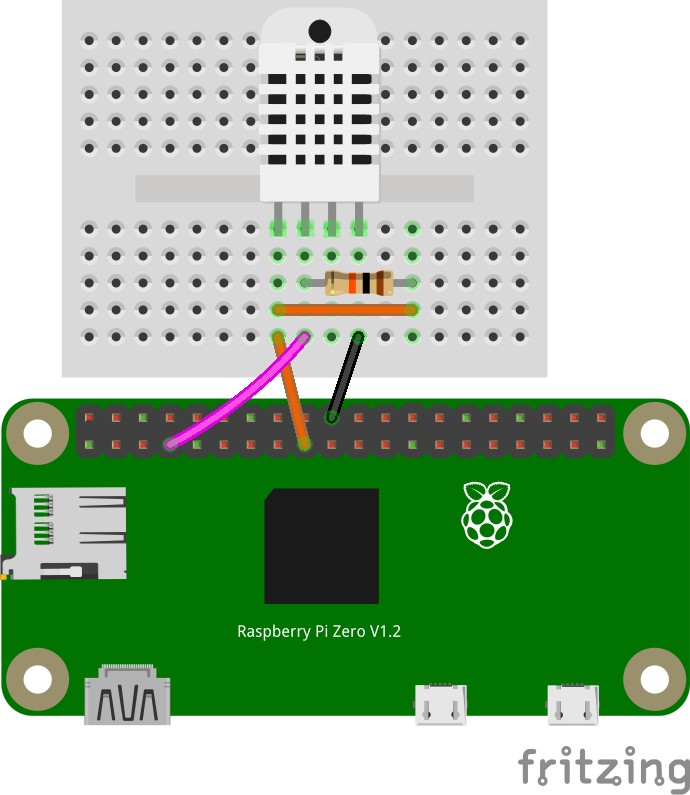
\includegraphics[scale=1.0, angle=-90]{images/DHT22_Steckplatine.png}	
  %	\caption{}
  \label{DHT22_Steckplatine}
\end{figure}

%\textbf{Schaltplan:} 

\begin{figure}[ht]
	\centering
	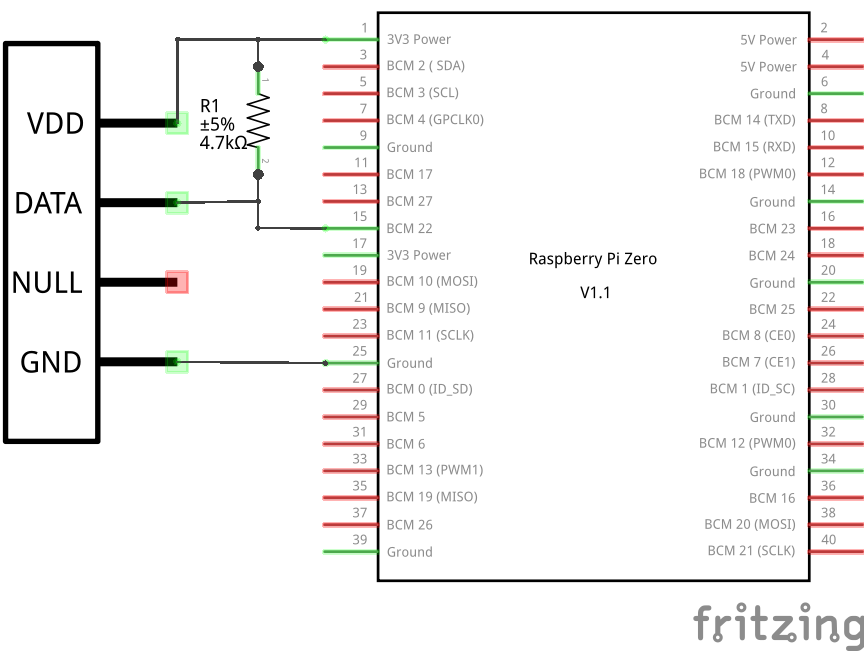
\includegraphics[scale=0.25]{images/DHT22_Schaltplan.png}	
	%	\caption{}
	\label{DHT22_Steckplatine}
\end{figure}


\textbf{C:}

\begin{console}
git clone https://github.com/mstroh76/Sensors-WiringPi.git
cd Sensors-WiringPi/DHT
g++ -o DHT *.cpp -lwiringPi	
sudo ./DHT 4
\end{console}

\textbf{Python:}
% Projektverzeichnis?
\begin{console}
git clone https://github.com/jdupl/dhtxx-rpi-python3.git
sudo cp dhtxx-rpi-python3/dhtxx.py /usr/local/lib/python3.5/dist-packages/
\end{console}

\lstset{language=Python, caption=, 
        label=DHT22Program, frame=single, basicstyle=\ttfamily
	      \footnotesize, breakatwhitespace=false, showstringspaces=false, 
        showtabs=false, tabsize=2 }
\lstinputlisting{source/DHT22.py}
